%%%%%%%%%%%%%%%%%%%%%%%%%%%%%%%%%%%%%%%%%%%%%%%%%%%%%%%%%%%%%%%
%PANDOC SPECIFIC SHIT, TAKEN FROM ANOTHER TEMPLATE...

\documentclass[11pt,]{article}

%Deal with margins and other geometry stuff
\usepackage[margin = 1in]{geometry}
\usepackage{longtable}
\usepackage{booktabs}

% Need to include this for refs with Pandoc

%Some of this is math package stuff, but honestly i don't really get
%what most of it is doing
\usepackage{amssymb,amsmath}
\usepackage{ifxetex,ifluatex}
\usepackage{fixltx2e} % provides \textsubscript

%Numbered section spacing
\setcounter{secnumdepth}{0}

\usepackage{setspace}
\setstretch{1}

%For LIST (enumerate) spacing
\providecommand{\tightlist}{%
  \setlength{\itemsep}{0pt}\setlength{\parskip}{0pt}}

%%%%%%%%%%%%%%%%%%%%%%%%%%%%%%%%%%%%%%%%%%%%%%%%%%%%%%%%%%%%%%%%%%%
%% LUCY'S DOCUMENT PREAMBLE AND PACKAGES

\usepackage{pdflscape}
\usepackage{xcolor}

\usepackage{tcolorbox}
\newtcolorbox{blackbox}{
  colback=white,
  colframe=black,
  coltext=black,
  boxsep=5pt,
  arc=4pt}

%\usepackage[round]{natbib}
\usepackage[sectionbib, natbibapa]{apacite} 
\usepackage[hyphens]{url}

%Set paragraph indent and between paragraph spacing
\usepackage{parskip}
\setlength\parindent{0pt}
\setlength{\parskip}{0pt}

%Need all these for graphics and tables
\usepackage{subfig}
\usepackage{graphicx}
\usepackage{blindtext}
\usepackage{array}
\usepackage{float}

%Deal with titles and make them less stupid and ugly
\usepackage{titlesec}
\titleformat{\section}[block]{\bfseries\sc\filcenter}{}{1em}{}
%\titleformat{\section}[block]{\Large\bfseries\filcenter}{}{1em}{}
\titleformat{\subsection}[hang]{\bfseries}{}{1em}{}
\setcounter{secnumdepth}{0}

\usepackage[hyphens]{url}

%Bunch of hyperlink shit
\usepackage{hyperref}
\hypersetup{
    colorlinks=true,
    linkcolor=blue,
    filecolor=magenta,      
    urlcolor=cyan,
    citecolor = black
}


%Header and footer junk
\usepackage{fancyhdr}
\pagestyle{fancy}
\fancyhead[L,C]{}
\fancyhead[R]{\small{\textsc{L E Delaney} \hspace{3mm} \textit{Chapter
1: Introduction to genetics}}}
\fancyfoot[L]{\tiny{\textit{Version date: \today}}}
    \fancyfoot[R]{\thepage}
\fancyfoot[C]{}


%%%%%%%%%%%%%%%%%%%%%%%%%%%%%%%%%%%%%%%%%%%%%%%%%%%%%%%%%%%%%%%%%%%%%%%
%% START OF THE DOCUMENT BODY
\begin{document}

%%%%%% TITLE 
\begin{center}
\Large{\textsc{Chapter 1: Introduction to
genetics}}\\ \small{\textit{Problems 1, 4, 5, 6, 10, 11, 12}}\\
\vspace*{\baselineskip}
\end{center}

%%%%%%%%%%%%%% DOCUMENT BODY
\begin{blackbox}

\begin{enumerate}
\def\labelenumi{\arabic{enumi}.}
\tightlist
\item
  If the white-flowered parental variety in Figure 1-3 were crossed to
  the first-generation hybrid plant in that figure, what types of
  progeny would you expect to see and in what proportions?
\end{enumerate}

\begin{center}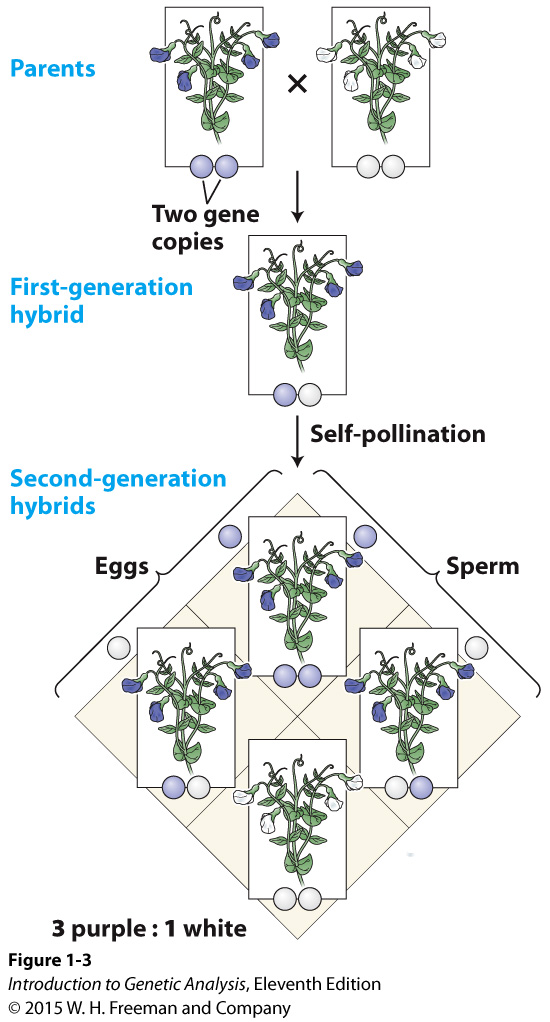
\includegraphics[width=0.35\linewidth,]{input/figure_01_03} \end{center}

\vspace{10mm}

\textbf{Answer}: Let's assign genotypes for each of these hypothetical
parents. First, we assign a genotype of AA to the purple plant, and aa
to the white plant. If a pure-breeding (homozygous) purple plant and a
pure-breeding (homozygous) white plant mated, we would observe the
following:

\[\begin{aligned}
AA \times aa \rightarrow Aa ~
\end{aligned}\]

Thus, all hybrid plants have a genotype of Aa. If we cross this to a
pure-breeding white-flowered plant (aa), we observe the following:

\begin{longtable}[]{@{}lll@{}}
\toprule
\begin{minipage}[b]{0.09\columnwidth}\raggedright
\strut
\end{minipage} & \begin{minipage}[b]{0.11\columnwidth}\raggedright
a\strut
\end{minipage} & \begin{minipage}[b]{0.11\columnwidth}\raggedright
a\strut
\end{minipage}\tabularnewline
\midrule
\endhead
\begin{minipage}[t]{0.09\columnwidth}\raggedright
A\strut
\end{minipage} & \begin{minipage}[t]{0.11\columnwidth}\raggedright
Aa\strut
\end{minipage} & \begin{minipage}[t]{0.11\columnwidth}\raggedright
Aa\strut
\end{minipage}\tabularnewline
\begin{minipage}[t]{0.09\columnwidth}\raggedright
a\strut
\end{minipage} & \begin{minipage}[t]{0.11\columnwidth}\raggedright
aa\strut
\end{minipage} & \begin{minipage}[t]{0.11\columnwidth}\raggedright
aa\strut
\end{minipage}\tabularnewline
\bottomrule
\end{longtable}

Like all single-locus crosses between a homozygote and heterozygote
(with complete dominance), we observe a 1:1 phenotypic and genotypic
ratio.

\end{blackbox}

\begin{blackbox}

\begin{enumerate}
\def\labelenumi{\arabic{enumi}.}
\setcounter{enumi}{3}
\tightlist
\item
  Figure 1-7 shows a simplified pathway for arginine synthesis in
  Neurospora. Suppose you have a special strain of Neurospora that makes
  citrulline but not arginine. Which gene(s) are likely mutant or
  missing in your special strain? You have a second strain of Neurospora
  that makes neither citrulline nor arginine but does make ornithine.
  Which gene(s) are mutant or missing in this strain?\\
\end{enumerate}

\begin{center}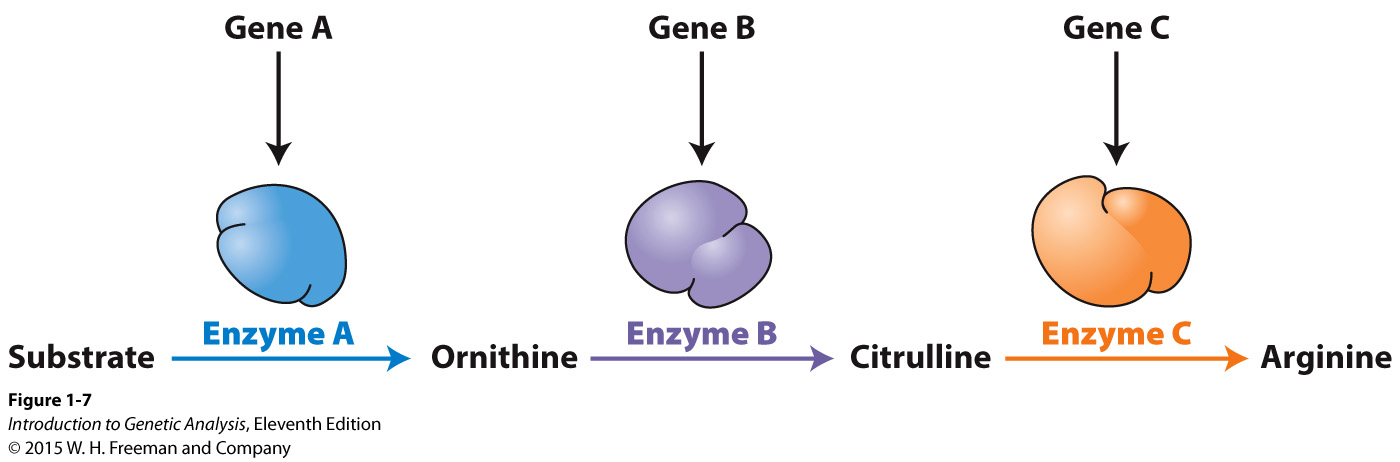
\includegraphics[width=0.45\linewidth,]{input/figure_01_07} \end{center}

\textbf{Answer}: If the mutant strain is able to produce citrulline,
then genes A and B must work. Gene C, the gene responsible for the
transition from citrulline to arginine, must be mutated.

In the second strain, gene A must be functional since it is able to make
ornithine. Gene B must be missing or mutant since it is unable to make
citrulline. However, gene C may or may not be missing or mutantated.
Enzyme C converts citrulline into arginine (they are in the same
sequential pathway), and enzyme C is dependent on the availability of
citrulline for its function.

\end{blackbox}

\begin{blackbox}
5. Consider Figure 1-8a. \begin{enumerate} 
 \item[a.]{ What do the small blue spheres represent? } 
 \item[b.]{ What do the brown slabs represent? } 
 \item[c.]{ Do you agree with the analogy that DNA is structured like a ladder? } 
 \end{enumerate}



\begin{center}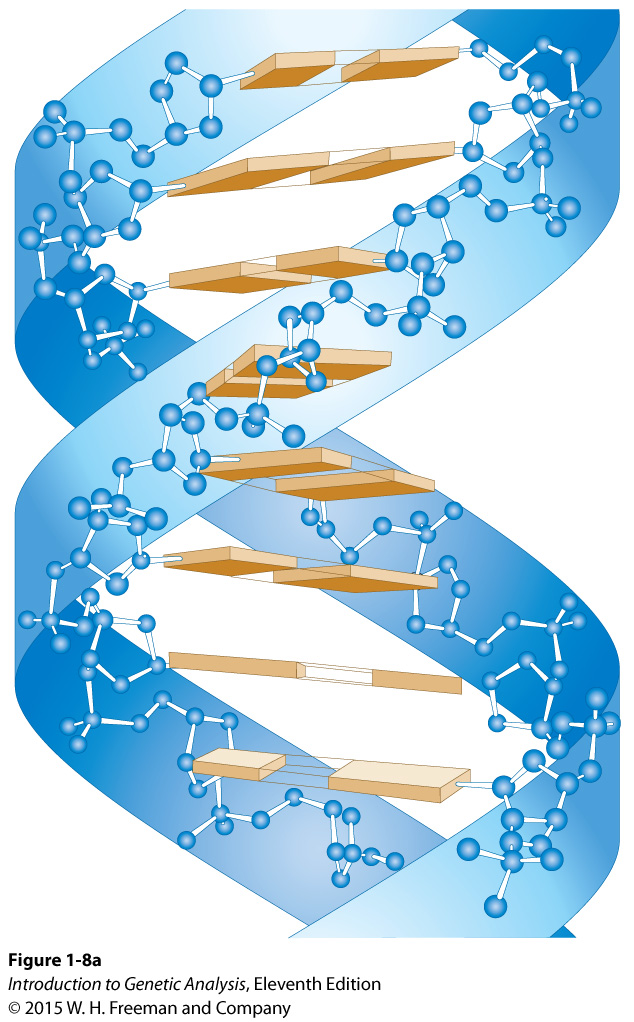
\includegraphics[width=0.25\linewidth,]{input/figure_01_08a} \end{center}

\textbf{Answer}:
\begin{enumerate} 
 \item[a.]{ The blue ribbon represents sugar phosphate backbone (deoxyribose and a phosphate group), while the blue spheres signify atoms } 
 \item[b.]{ Brown slabs show complementary bases (A, T, G, and C) } 
 \item[c.]{ Yes, it is a helical structure } 
 \end{enumerate}
\end{blackbox}

\begin{blackbox}

\begin{enumerate}
\def\labelenumi{\arabic{enumi}.}
\setcounter{enumi}{5}
\tightlist
\item
  In Figure 1-8b, can you tell if the number of hydrogen bonds between
  adenine and thymine is the same as that between cytosine and guanine?
  Do you think that a DNA molecule with a high content of A + T would be
  more stable than one with a high content of G + C?
\end{enumerate}

\begin{center}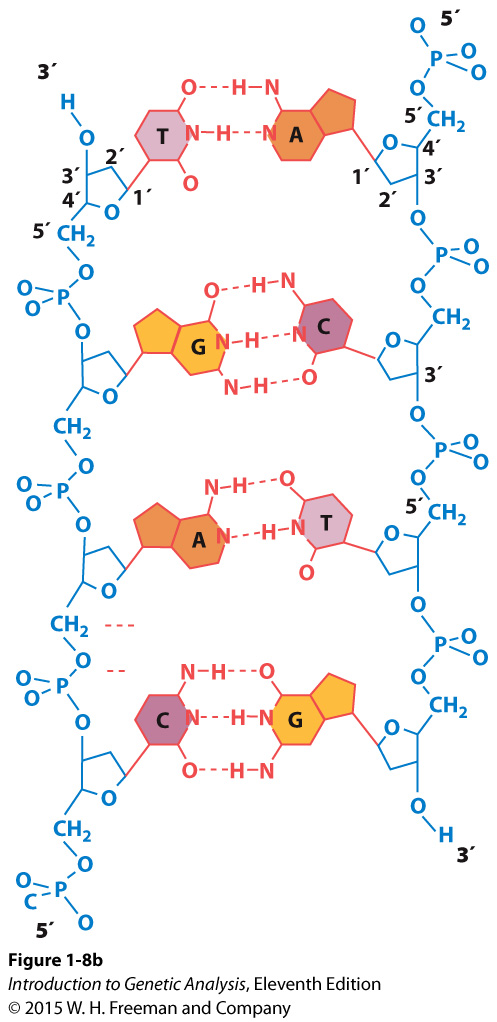
\includegraphics[width=0.25\linewidth,]{input/figure_01_08b} \end{center}

\textbf{Answer:} There are two hydrogen bonds between adenine and
thymine and three between guanine and cytosine. Because A-T has only two
hydrogen bonds it will be less stable than a molecule with a high
content of G-C (three hydrogen bonds).

\end{blackbox}

\begin{blackbox}

\begin{enumerate}
\def\labelenumi{\arabic{enumi}.}
\setcounter{enumi}{9}
\tightlist
\item
  Below is the sequence of a single strand of a short DNA molecule. On a
  piece of paper, rewrite this sequence and then write the sequence of
  the complementary strand below it.
\end{enumerate}

\vspace{10mm}

GTTCGCGGCCGCGAAC

\vspace{10mm}

Comparing the top and bottom strands, what do you notice about the
relationship between them?

\vspace{10mm}

\textbf{Answer:}

GTTCGCGGCCGCGAAC

CAAGCGCCGGCGCTTG

They are palindromes --- the same forwards and backwards.

\end{blackbox}

\begin{blackbox}

11. Mendel studied a tall variety of pea plants with stems that are 20 cm long and a dwarf variety with stems that are only 12 cm long. \begin{enumerate} 
 \item[a.]{ Under blending theory, how long would you expect the stems of first and second hybrids to be? } 
 \item[b.]{ Under Mendelian rules, what would you expect to observe in the second-generation hybrids if all the first-generation hybrids were tall? } 
 \end{enumerate}

\vspace{10mm}

\textbf{Answer}: 
\begin{enumerate} 
 \item[a.]{ Blending theory suggests that offspring would exhibit traits in between both parents, i.e., the average. In this case, offspring would be 16cm tall. } 
 \item[b.]{ If all F1 hybrids were tall, this suggests that tall is dominant to short and all offspring are heterozygous. Thus, upon mating F1 hybrids, you would expect a 3:1 ratio of tall to short. } 
 \end{enumerate}

\end{blackbox}

\begin{blackbox}

\begin{enumerate}
\def\labelenumi{\arabic{enumi}.}
\setcounter{enumi}{11}
\tightlist
\item
  If a DNA double helix that is 100 base pairs in length has 32
  adenines, how many cytosines, guanines, and thymines must it have?
\end{enumerate}

\vspace{10mm}

\textbf{Answer:}

A = T and G = C. Therefore, 32 adenines means there are also 32
thymines, for a total of 64 bases. This means the remainder (100 - 64 =
36) are guanines and cytosines. Split 36 in two because the number of Gs
and Cs are equal, and you get 18 guanine and 18 cytosine.

\end{blackbox}

\end{document}


